\section{Linear regression}

%% Function approximation with least squares {{{
\subsection{Function approximation with least squares}


\subsubsection*{Ordinary least-squares}

At first, a noisy sample of $x\,\rightarrow\,y$ is generated.
Let $[\v{\Phi}]_{ij}=\fn{f}_j(x_i)$ be the transformed input vector and $\v{y}$ the output,
where $\fn{f}_j$ is a basis function. We have to find the $\v{\theta}$ parameter vector,
for which $\v{\Phi}\,\v{\theta}=\v{y}$. From this the $\v{\Phi}(x)$ matrix can be generated
after selecting a suitable $\fn{f}$. A number of these were tried, and the best one
seemed to be the polynomial one, that is $\fn{f}_{i}(x) = x^{i-1}$.
As a parameter, $d=10$ was used.
The $\v{\Phi}$ matrix of the sampled inputs and of the LS estimate are the same,
so the function is evaluated at the same $x$ values.

For the QR decomposition problem, the ''economic'' mode of scipy's \verb|qr| function
is used, then $\hat{\v{\theta}}$ is found with $\hat{\v{\theta}} = \v{R}^{-1}\v{Q}\T\v{y}$.
Because the pseudoinverse of a matrix is unique,
this method gives the same result as the previous one.

The results are shown in figure \ref{fig:ex_I_1_plots_1}.

\subsubsection*{Recursive least-squares}

% Next, more of the above described $(x, y)$ pairs is sampled and $\hat{\v{\theta}}_{n}$ calculated periodically using recursive least-squares. In the code, all of the samples are measured beforehand for simplicity.
The equation for $\hat{\v{\theta}}$ can be reformulated in the following way:
\begin{equation}
	\hat{\v{\theta}} = \underbrace{\left[\sum\limits_{i=1}^n{\v{\varphi}\,\v{\varphi}\T}\right]^{-1}}_{\v{\Psi}_n}\,
	\underbrace{\sum\limits_{i=1}^n{y_{i}\,\v{\varphi}_{i} }}_{z_n}.
\end{equation}
Now we have an update rule for both $\v{\Psi}_{n+1} = \brc{\v{\Psi} + \v{\varphi}_{n+1}\v{\varphi}_{n+1}\T}^{-1}$, and $z_{n+1} = z_n + \v{\varphi}_{n+1}\v{y}_{n+1}$.
Both $\v{\Psi}_0$ and $z_0$ are set to zero. 
Also, in the code $\v{\theta}_n$ is calculated only when plotted for speed.

The resulting plots are shown in figure \ref{fig:ex_I_1_plots_2}.,
taken at $n\in[25, 50, 75, 100]$.

\subsubsection*{Least-norm problem}

Now let's make $d>n$, which makes $\v{\Phi}$ fat, specifically $n=100$ and $d=200$.
We make the assumption that $\v{\Phi}$ is still full-rank.
The solution is the same, except we are going to use singular value decomposition (SVD)
for the pseudoinverse of $\v{\Phi}$.

The SVD is calculated like this: $\v{\Phi}_{d\times n}=\v{U}_{d\times d}\,\v{\Sigma}_{d\times n}\,\v{V}_{n\times n}\T$. Let's denote the matrix of column vectors of the normalized eigen-vectors 
of matrix $\v{\Phi}$ by $\eig(\v{\Phi})$. Let's denote the eigenvalues by $\operatorname{eigval}(\v{\Phi})$.
Then, $\v{U} = \eig(\v{\Phi}\,\v{\Phi}\T)$, $\v{V} = \eig(\v{\Phi}\T\,\v{\Phi})$ and
$\v{\Sigma} = \diag(\operatorname{eigval}(\v{\Phi}\,\v{\Phi}\T))_{d\times n}$.
Then, the pseudoinverse is $\v{\Phi}^+=\v{V}\,\v{\Sigma}^+\,\v{U}\T$.
For $\v{\Sigma}^+$, we take the inverse of the non-zero elements of $\v{\Sigma}$, and add
zeros such that it has the shape of $d\times n$.

The resulting plots are shown in figure \ref{fig:ex_I_1_plots_3}.

\begin{figure}[H]
	\centering
	\begin{subfigure}[b]{.43\textwidth}
		\centering
		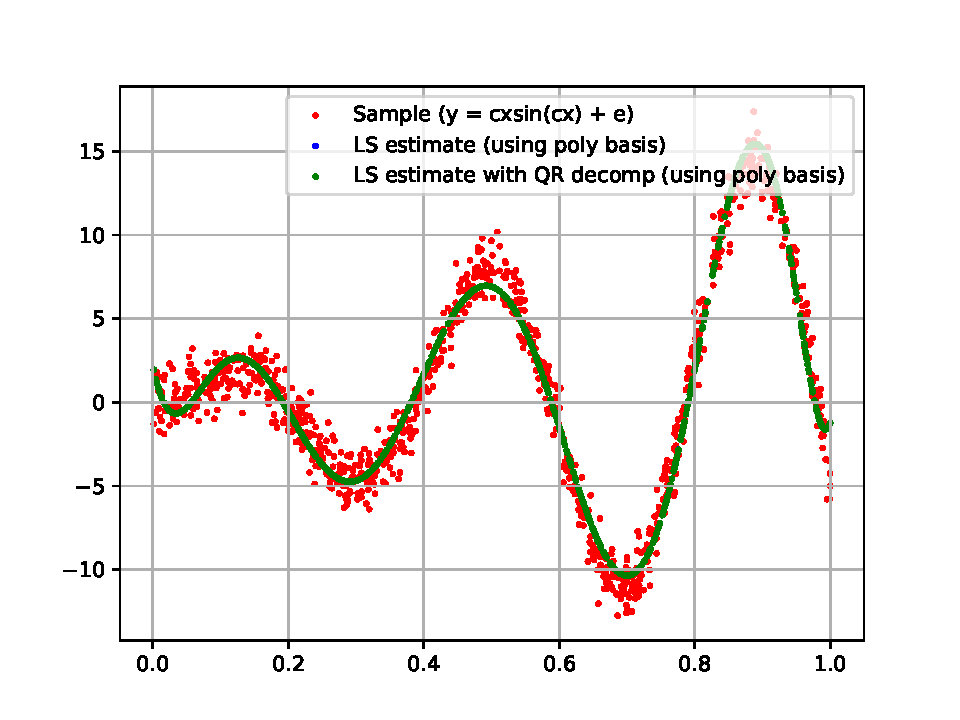
\includegraphics[width=\textwidth, trim={10mm, 2mm, 15mm, 10mm}, clip]{ex_I_1_plots_1}
		\caption{Least-squares estimate for thin $\v{\Phi}$}
		\label{fig:ex_I_1_plots_1}
	\end{subfigure}\hfill
	\begin{subfigure}[b]{.43\textwidth}
		\centering
		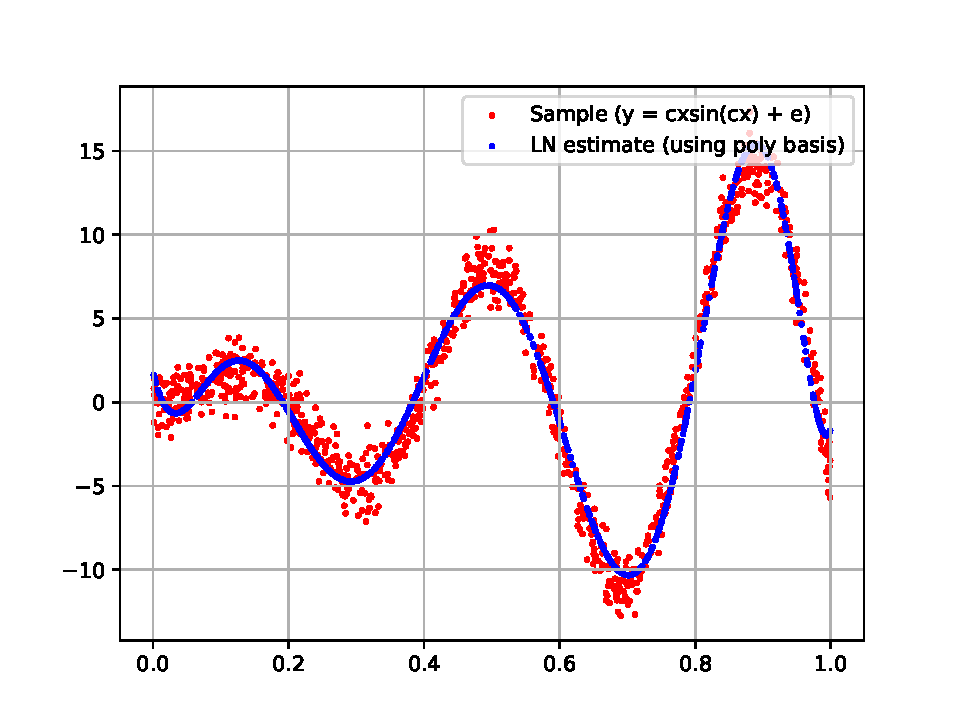
\includegraphics[width=\textwidth, trim={10mm, 2mm, 15mm, 10mm}, clip]{ex_I_1_plots_3}
		\caption{Least-norm estimate for fat $\v{\Phi}$}
		\label{fig:ex_I_1_plots_3}
	\end{subfigure}\\
	\begin{subfigure}[b]{.45\textwidth}
		\centering
		\vspace{6mm}
		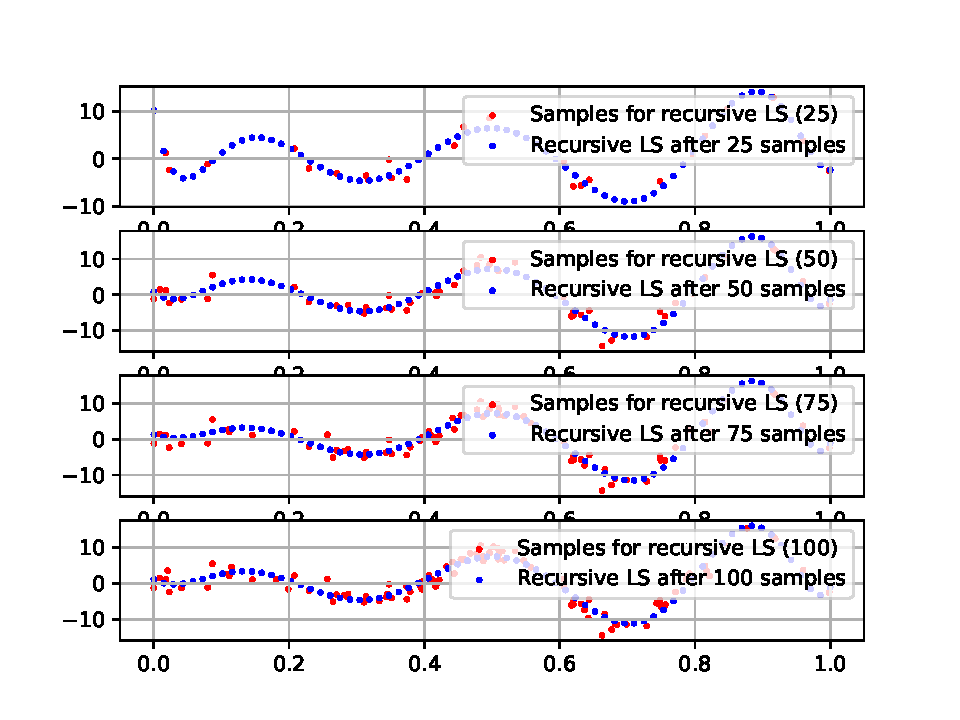
\includegraphics[width=\textwidth, trim={20mm, 2mm, 15mm, 10mm}]{ex_I_1_plots_2}
		\caption{Recursive least-squares}
		\label{fig:ex_I_1_plots_2}
	\end{subfigure}
	\caption{Experiments with ordinary least-squares}
\end{figure}

%% }}}

%% Approximating auto-regressive series {{{
\subsection{Approximating auto-regressive series}

A recursive time-series is generated from the give equation: $y_t = a\,y_{t-1} + b\,y_{t-2} + \epsilon_t$.

\begin{figure}[H]
	\centering
	\begin{subfigure}[b]{.49\textwidth}
		\centering
		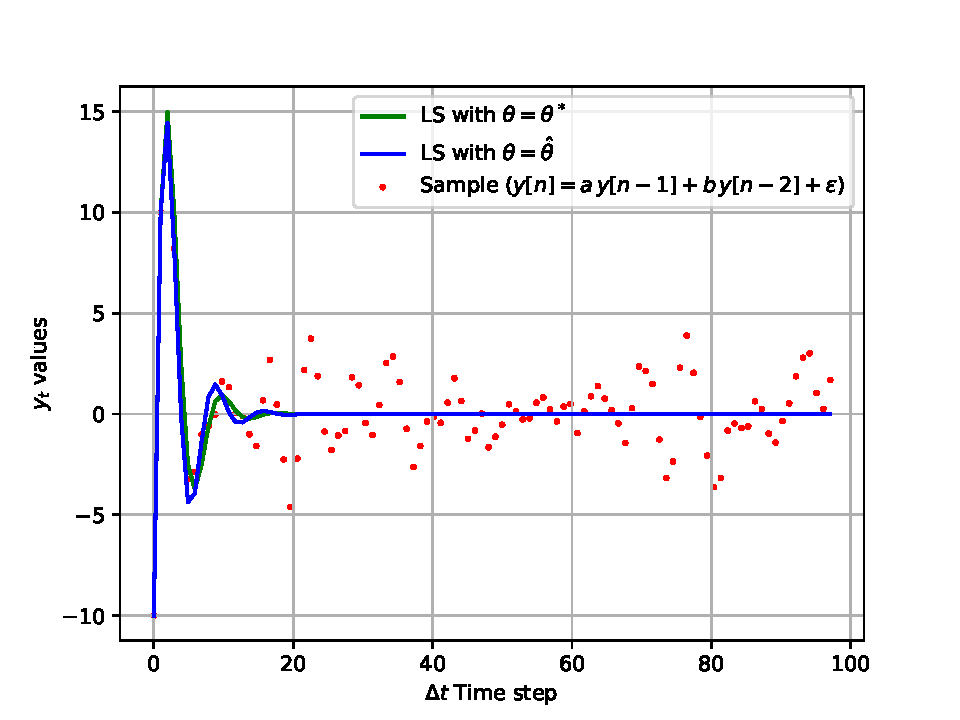
\includegraphics[width=\textwidth, trim={5mm, 2mm, 15mm, 10mm}, clip]{ex_I_2_plots_1}
		\caption{}
		\label{fig:ex_I_2_plots_1}
	\end{subfigure}\hfill
	\begin{subfigure}[b]{.49\textwidth}
		\centering
		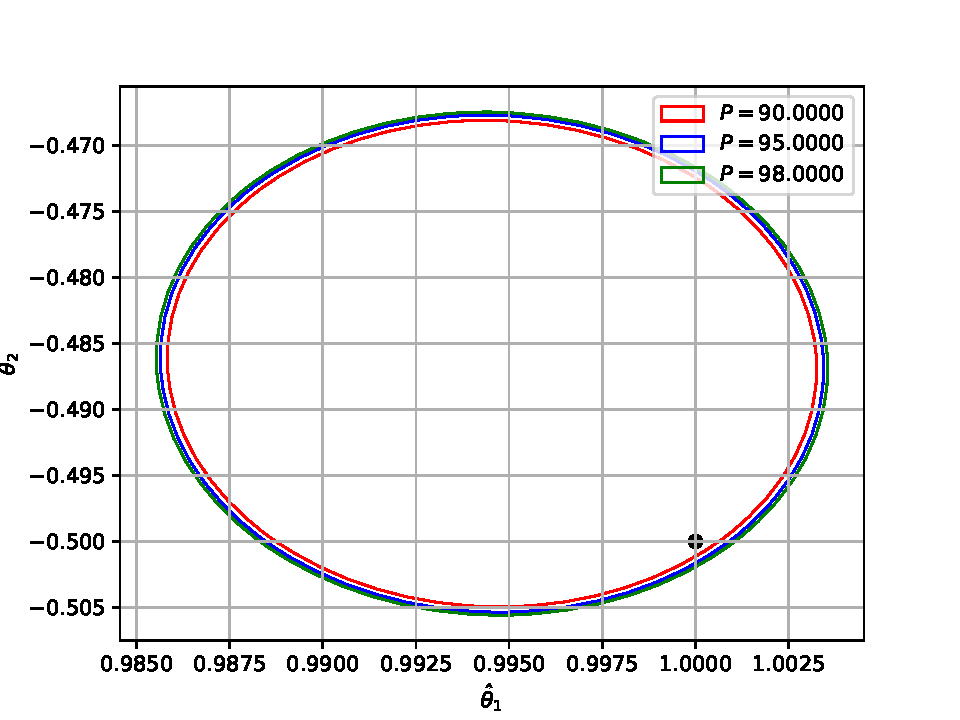
\includegraphics[width=\textwidth, trim={0mm, 2mm, 15mm, 10mm}, clip]{ex_I_2_plots_2}
		\caption{}
		\label{fig:ex_I_2_plots_2}
	\end{subfigure}
\end{figure}

%% }}}
